
\begin{figure}[H]
 \begin{center}
   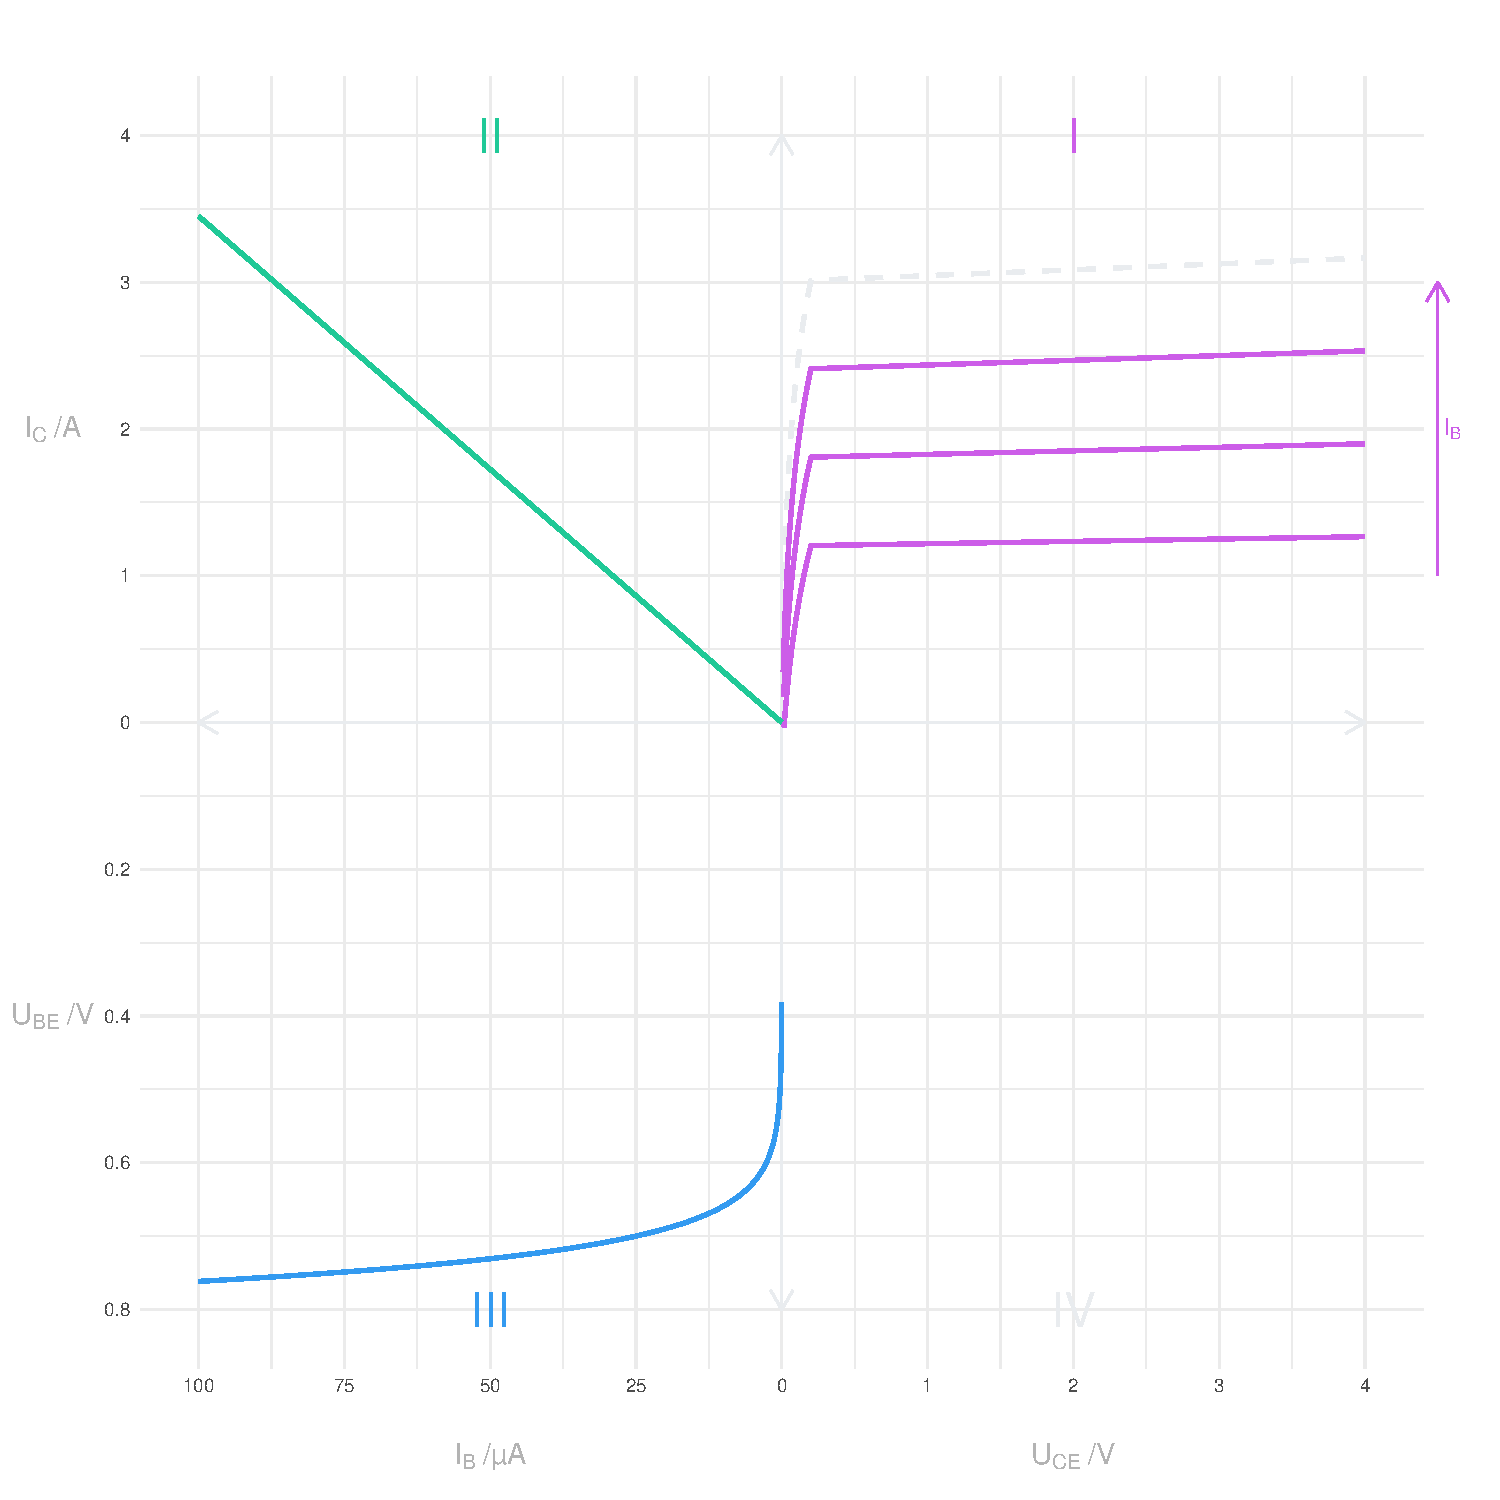
\includegraphics[width=\textwidth]{1_2/2_1_4Q}
 \end{center}
\end{figure}
\subsubsection{I: Ausgangskennlinienfeld}
\textcolor{grape5}{Quadrant I} stellt die Abhängigkeit des Kollektorstroms $I_C$ von der
Kollektor-Emitter-Spannung $U_{CE}$ dar. Da diese zusätzlich vom
Basisstrom $I_B$ abhängig ist, können einzelne Kennlinien nur für ausgewählte Werte
von $I_B$ angegeben werden, es ergibt sich das Ausgangskennlinienfeld. Das
Kennlinienfeld beginnt bei fortlaufender Kollektorspannung mit dem Transistor im
Sättigungsbetrieb, da die Basis-Emitter-Spannung > $0 \, \si{\volt}$ und die
Basis-Kollektor-Spannung ebenfalls > $0 \, \si{\volt}$ ($U_{BC} = U_{BE} -
U_{CE}$) ist. Beide pn-Übergänge sind in Durchlassrichtung gepolt, wodurch der
Kollektorstrom mit kleiner werdender Kollektor-Emitter-Spannung $U_{CE}$
abnimmt. Dies ist nicht der Normalbetriebsfall, weshalb die statische Stromverstärkung
$B_N$ in diesem Bereich nicht gilt. Den Bereich ab etwa $U_{CE} = 0.6 \,
\si{\volt}$ bezeichnet man als aktiven Vorwärtsbetrieb.

\subsubsection{II: Stromsteuerkennlinie}
\textcolor{teal5}{Quadrant II} zeigt den Zusammenhang zwischen Eingangsstrom $I_B$
und Ausgangsstrom $I_C$. Das Verhalten ist bis auf die Bereiche sehr großer und
sehr niedriger Ströme annäherungsweise linear. Der statische Verstärkungsfaktor
$B_N$ (Gleichstromverstärkungsfaktor) kann daher als
\[B_N=\frac{I_C}{B_N}\]
ausgedrückt werden (gilt nur für \emph{einen} statisch eingestellten Arbeitspunkt).

\subsubsection{III: Eingangskennlinienfeld}
Im \textcolor{blue5}{Quadranten III} kann durch Verfolgen der Eingangsgrößen
Basis-Spannung $U_{BE}$ und -Strom $I_B$ das Diodenverhalten des
Basis-Emitter-pn-Übergangs erkannt werden.

\subsubsection{IV: Rückwirkungskennlinienfeld}
\textcolor{gray7}{Quadrant IV} stellt die Rückwirkung der
Kollektor-Emitter-Spannung auf die Basis-Emitter-Spannung dar, meist beschränkt
man sich jedoch auf die Quadranten I, II und III.